\chapter{Research design}\label{chap:research}

\section{Mathematical Constraints}

The objective of the mathematical model is to build a Thread network that adheres to specific mathematical constraints, ensuring a well-functioning network with the optimum device types, sensitivity, and RSSI. By complying with the constraints, the Thread network can be effectively optimized for both performance and energy consumption. The constraints of the model are as follows:

\begin{enumerate}
    \item To establish a link between the sensors and EDs, the RSSI of each end device must be approximately above the sensitivity of each ED. This ensures a stable connection between the devices \cite{wu2014study}.
    \item The transmission power limitation, ranging from -20 dBm to 8 dBm, is set according to the hardware specifications of the devices in the Thread network, ensuring optimal performance while facilitating power optimization techniques within these constraints for energy efficiency \cite{semiconductor_nrf52840_2018_1}.
    \item The number of REEDs must be equal to the number of routers and the leader because, if a router is lost, a connected REED must become a router to replace the dead router and maintain network resilience.
    \item To establish a connection between the EDs and routers, the RSSI of each router must be approximately above the sensitivity of each router. This guarantees a stable link between the devices and the routers \cite{wu2014study}.
    \item To establish a connection between the routers and border routers, the RSSI of each border router must be approximately above the sensitivity of each border router, ensuring a reliable link between the network components \cite{wu2014study}.
\end{enumerate}

The following mathematical model is designed for this purpose:

\begin{equation}\label{eq:minimize_power}
    \begin{aligned}
        Min\sum_{i=1}^{M}P_t^i
    \end{aligned}
\end{equation}

\textbf{Subjects to:}
\begin{equation}\label{eq:mathematical_constraints_end_device}
    \begin{split}
        RSSI_{ED}^j>EDSensitivity,j\in1,\cdots,N \\
        -20dBm{\le P}_t^j\le8dBm \\
        N_{REED}=n_{Router}+n_{Leader} \\
    \end{split}
\end{equation}

\begin{equation}\label{eq:mathematical_constraints_router}
    \begin{split}
        {RSSI}_{Router}^k>RouterSensitivity,k\in1,\cdots,O \\
        -{20dBm\le P}_t^k\le8dBm
    \end{split}
\end{equation}

\begin{equation}\label{eq:mathematical_constraints_border_router}
    \begin{split}
        {RSSI}_{BD}^L>BDSensitivity,L\in1,\cdots,P \\
        -{20dBm\le P}_t^L\le8dBm \\
        Sensitivity=-100dBm \\
        SEED\in0,1 \\
        n_{Leader}=1 \\
        n_{Router}+n_{Leader}\geq3 \\
        n_{BR}=2
    \end{split}
\end{equation}

Where $P_t$ represents the Transmit Power of each one of the $M$ devices, $RSSI$ is the Received Signal Strength Intensity, $ED$ is End Device, $REED$ is Router Eligible End Devices, $N_{REED}$ is the number of the REEDs, $n_{Router}$ is the number of the routers, $n_{Leader}$ is number of the leaders, $N$ is amount of end devices, $O$ is the number of Routers, $P$ is the number of Border Routers, $SEED$ is Sleepy End Devices, and $Sensitivity$ is $-100 dBm$ with IEEE 802.15.4 \cite{Semiconductor_Nordic_Product_Brief_2018_2.0}.

\section{Monte Carlo Method Process}\label{sec:monte_carlo_method_process}

The Monte Carlo Method involves four main steps. First, the process is initialized with predefined parameters and constraints. Second, random numbers are generated within the defined bounds to explore various network configurations. Third, the generated configurations are evaluated based on their performance and adherence to constraints. Finally, after a predetermined number of iterations or reaching an acceptable solution, the MCM process comes to an end, providing an optimized network configuration. For a detailed explanation of each step, refer to the respective sections below.

\subsection{Initialize}

The Monte Carlo method is initiated to optimize the Thread network, considering the key parameters influencing the network's performance and energy efficiency. These parameters are outlined in the table below:

\begin{longtable}{>{\hspace{0pt}}m{0.098\linewidth}>{\hspace{0pt}}m{0.842\linewidth}}
    \label{tab:monte_carlo_parameters}\\
    \caption{Parameters influencing Monte Carlo Method.}\\
    \hline\hline
    Param & Description
    \endfirsthead
    \hline
    $N_d$     & The total number of devices participating in the network, which is set to 8 for this research, representing a small-scale IoT network.                                                                              \\
    $P_{tx}$  & Determines the signal strength for each device, randomly generated in a range between -20 $dBm$ and 8 $dBm$ according to the mathematical constraints, affecting network connectivity and energy consumption.       \\
    $F_c$     & The carrier frequency used for calculating RSSI using the general path loss model, set at 2.4 ${GH}_z$, based on Thread protocol specification.                                                                     \\
    $D_0$     & A reference distance of 0.25 $m$, associated with the carrier frequency $F_c$, employed in the path loss model to calculate signal attenuation.                                                                     \\
    $d$       & Represents the distance between two devices in the network, as illustrated in figures \ref{fig:distance_matrix_lab} and \ref{fig:distance_matrix_home}, influencing the strength of the signal received by devices. \\
    $n$       & The path loss exponent, set to 5.0, which represents the rate at which the signal power decays with distance in the path loss model.                                                                                \\
    $\sigma$  & The variance of the shadowing component, set to 3.0 $dB$, accounts for signal fluctuations due to obstacles and multipath propagation in the environment.                                                           \\
    $G_t$     & The transmit antenna gain, set to 0.0 $dB$, which reflects the effectiveness of the transmitting antenna in directing the radio waves towards the receiving device.                                                 \\
    $G_r$     & The receive antenna gain, set to 0.0 $dB$, indicating the receiving antenna's ability to capture incoming radio waves.                                                                                              \\
    \hline\hline
\end{longtable}

\subsection{Generate Random Numbers}

Based on the factors mentioned at the start, MCM generates a vector $X$ of length equal to $2n$, where $n$ is the number of places where network elements can be allocated \cite{1576539}. The vector is represented as:

\begin{equation}\label{eq:vector_x}
    \begin{split}
        X=\left[x_1,x_2,x_3,\cdots x_n,p_1,p_2,p_3,\cdots,p_n\right] \\
        for{\ x}_n\in0,1,2,3,4,5 \\
        p_n\in-20:4:8\ dBm
    \end{split}
\end{equation}

    Where $0$ represents no element allocated, $1$ is allocate a SEED, $2$ is allocate a REED, $3$ is allocate a Router, $4$ is allocate the Leader, and $5$ is allocate a Border Router.
\vspace{2mm}

\subsection{Evaluate Results}

The objective function aims to build a Thread network using the optimal network configuration without violating the mathematical constraints. If a constraint is violated, a penalty is added to the objective function, which is weighted according to the importance of the constraint. The objective function with penalty values can be written as:

\begin{equation}\label{eq:objective_function}
    \begin{aligned}
        Min\sum_{i=1}^{M}P_t^i+penal_1+penal_2+penal_3\ldots+penal_{nr}
    \end{aligned}
\end{equation}

    Where $penal_1$ represents penalty for violating the first restriction, $penal_2$ is penalty for violating the second restriction, and $penal_{nr}$ is the penalty for violating the last restriction.
\vspace{2mm}

\subsection{Termination}

The MCM converges on an optimal solution that satisfies necessary constraints, providing outputs such as device types, transmission power, and position. It also offers information on constraint violations, including the penalty, power consumption, and RSSI sensitivity violations—these outputs aid in understanding the optimization process and refining the network design. For a comprehensive understanding of the four steps of the MCM process, refer to the following pseudocode, which provides an overview of the algorithm's structure and logic.

\begin{algorithm}[H]
    \caption{Monte Carlo Method pseudocode for network optimization.}
    \label{alg:mcm}
    \begin{algorithmic}
    \STATE Initialize MCM parameters: $N_d$, $d$, $F_c$, $D_0$, $n$, $\sigma$, $G_t$, $G_r$
    \WHILE{network}
        \STATE devices, txpower, position $\gets$ generate\_random\_numbers($N_d$)
        \STATE penalty, path\_loss, rssi\_uplink, rssi\_downlink $\gets$ mathematical\_constraints\_evaluation($N_d$, $d$, $F_c$, $D_0$, $n$, $\sigma$, $G_t$, $G_r$)
        \IF{penalty is False}
            \STATE network $\gets$ False
        \ENDIF
        \RETURN devices, txpower, penalty, path\_loss, rssi\_uplink, rssi\_downlink
    \ENDWHILE
    \end{algorithmic}
\end{algorithm}

It is a simplified version of the Monte Carlo Method implementation and does not cover all the details of the original code. It is focused on the primary structure and steps of the method for network optimization and initial network build-up transmission power. To access the complete version of the algorithm code, including all implementation details, refer to the appendix \ref{appendix} section.

\section{Genetic Algorithm Process}\label{sec:genetic_algorithm}

The Genetic Algorithm process can be summarized into four main steps: initializing population, evaluating fitness, performing selections, and finding the best solution. These steps are designed to optimize transmission power in the network by evolving a population of candidate solutions through generations. In the following paragraphs, each step is discussed in detail.

\subsection{Initialize}

The initial steps of the GA process start with creating a random population with the specified population size, representing different possible network configurations. The population is generated based on the parameters set, as shown below:

\begin{longtable}{>{\hspace{0pt}}m{0.077\linewidth}>{\hspace{0pt}}m{0.865\linewidth}}
    \label{tab:ga_parameters}\\
    \caption{Parameters influencing Genetic Algorithm.}\\
    \hline\hline
    Param            & Description \endfirsthead
    \hline
    Population size  & The number of individuals in the population representing different possible network configurations are set to 100 for this research.                                                                                                                                                                                             \\
    Population       & An initial random population is created with the specified population size and MCM output, which includes device types, transmission power, and device positions, representing different possible network configurations. For instance: [ [3, 5, 2, 5, 1, 5, 0, 0], [-20, 0, 0, -8, 0, -12, 0, -20], [1, 2, 3, 4, 5, 6, 7, 8]].  \\
    Max iteration    & The maximum number of iterations to be performed by the Genetic Algorithm, for instance, 100 in this research.                                                                                                                                                                                                                   \\
    Mutation rate    & The probability of mutation is set at 0.1 for this research, determining the frequency of random changes introduced to the offspring's genetic information during the optimization process, which helps maintain genetic diversity within the population.                                                                        \\
    Selection method & The method used for selecting individuals from the current population to create the next generation, such as roulette wheel selection, tournament, or sorted. In this research, the sorted selection method was utilized.                                                                                                        \\
    Mutation method  & The method used for mutating individuals affect how genetic information is altered during the mutation process. In this research, the swap mutation method was utilized.                                                                                                                                                         \\
    \hline\hline
\end{longtable}

\subsection{Evaluate Fitness}

For each candidate in the population, calculate its fitness score. The fitness measures how effectively the configuration optimizes power consumption, considering path loss and RSSI sensitivity. Lower power consumption results in a higher fitness value, helping the algorithm identify the best individuals for producing the next generation.

\subsection{Selection, Crossover, and Mutation}

In this step, parents are selected from the current population based on their fitness values using sorted selection method. This ensures that individuals with higher fitness values have a higher chance of being chosen as parents, promoting the selection of potentially better solutions.

Next, the crossover operation is performed on the selected parents to create offspring by exchanging genetic material between pairs of parents. The crossover process combines the characteristics of parent individuals, allowing the offspring to inherit properties from both parents, which helps explore new potential solutions in the search space.

Finally, the mutation operation introduces small random changes to the offspring's genetic material by flipping bits within a certain probability (mutation rate). This process enhances diversity within the population and helps to prevent the algorithm from converging prematurely to suboptimal solutions by maintaining variation and allowing the exploration of alternative search paths.

\subsection{Population Update and Termination}

After the selection, crossover, and mutation processes, the new offspring are evaluated for their fitness. The population is then updated by replacing all individuals in the current population with the newly generated offspring. This step ensures that the best solutions found so far are preserved and that the overall fitness of the population improves over time.

The GA process iterates through the aforementioned steps for a predefined number of iterations. Once the termination criteria are met, the algorithm returns the best solution found throughout the entire evolutionary process, representing the most optimal network configuration discovered by the GA. Refer to the following pseudocode for an algorithmic overview of the Genetic Algorithm process:

\begin{algorithm}[H]
    \caption{Genetic Algorithm pseudocode for transmission power optimization.}
    \label{alg:genetic_algorithm}
    \begin{algorithmic}[1]
    \STATE Initialize GA parameters: population\_size, population, max\_iterations, mutation\_rate, selection\_method
    \STATE Initialize population: create\_random\_population(population\_size)
    \FOR{each candidate in population}
        \STATE fitness = evaluate\_fitness(candidate)
    \ENDFOR
    \FOR{generation in range(max\_iterations)}
        \STATE parents = select\_parents(population, selection\_method)
        \STATE offspring = crossover(parents, crossover\_prob)
        \STATE offspring = mutate(offspring, mutation\_prob)
        \FOR{each candidate in offspring}
            \STATE fitness = evaluate\_fitness(candidate)
        \ENDFOR
        \STATE population = replace\_population(population, offspring)
    \ENDFOR
    \STATE best\_solution = find\_best\_solution(population)
    \end{algorithmic}
\end{algorithm}

The output is a list of optimized transmission power values for each device, along with device types, positions, and penalty values. For a comprehensive understanding of the Genetic Algorithm's implementation, refer to the appendix \ref{appendix} for the complete code.

\section{Experimental Setup}

The prototype was built to validate the output from MCM and GA, using the optimal network configuration determined by MCM, which consisted of a total of 8 devices. The setup included 2 border routers, 3 routers (with one of them automatically elected as a leader), and 3 REEDs. The prototype was designed to closely resemble the conceptual model presented earlier in the figure, with the only slight difference being the use of REEDs instead of sensors as the end devices. An image was provided below to illustrate the Thread network topology that had been constructed.

\begin{figure}[H]
    \centering
    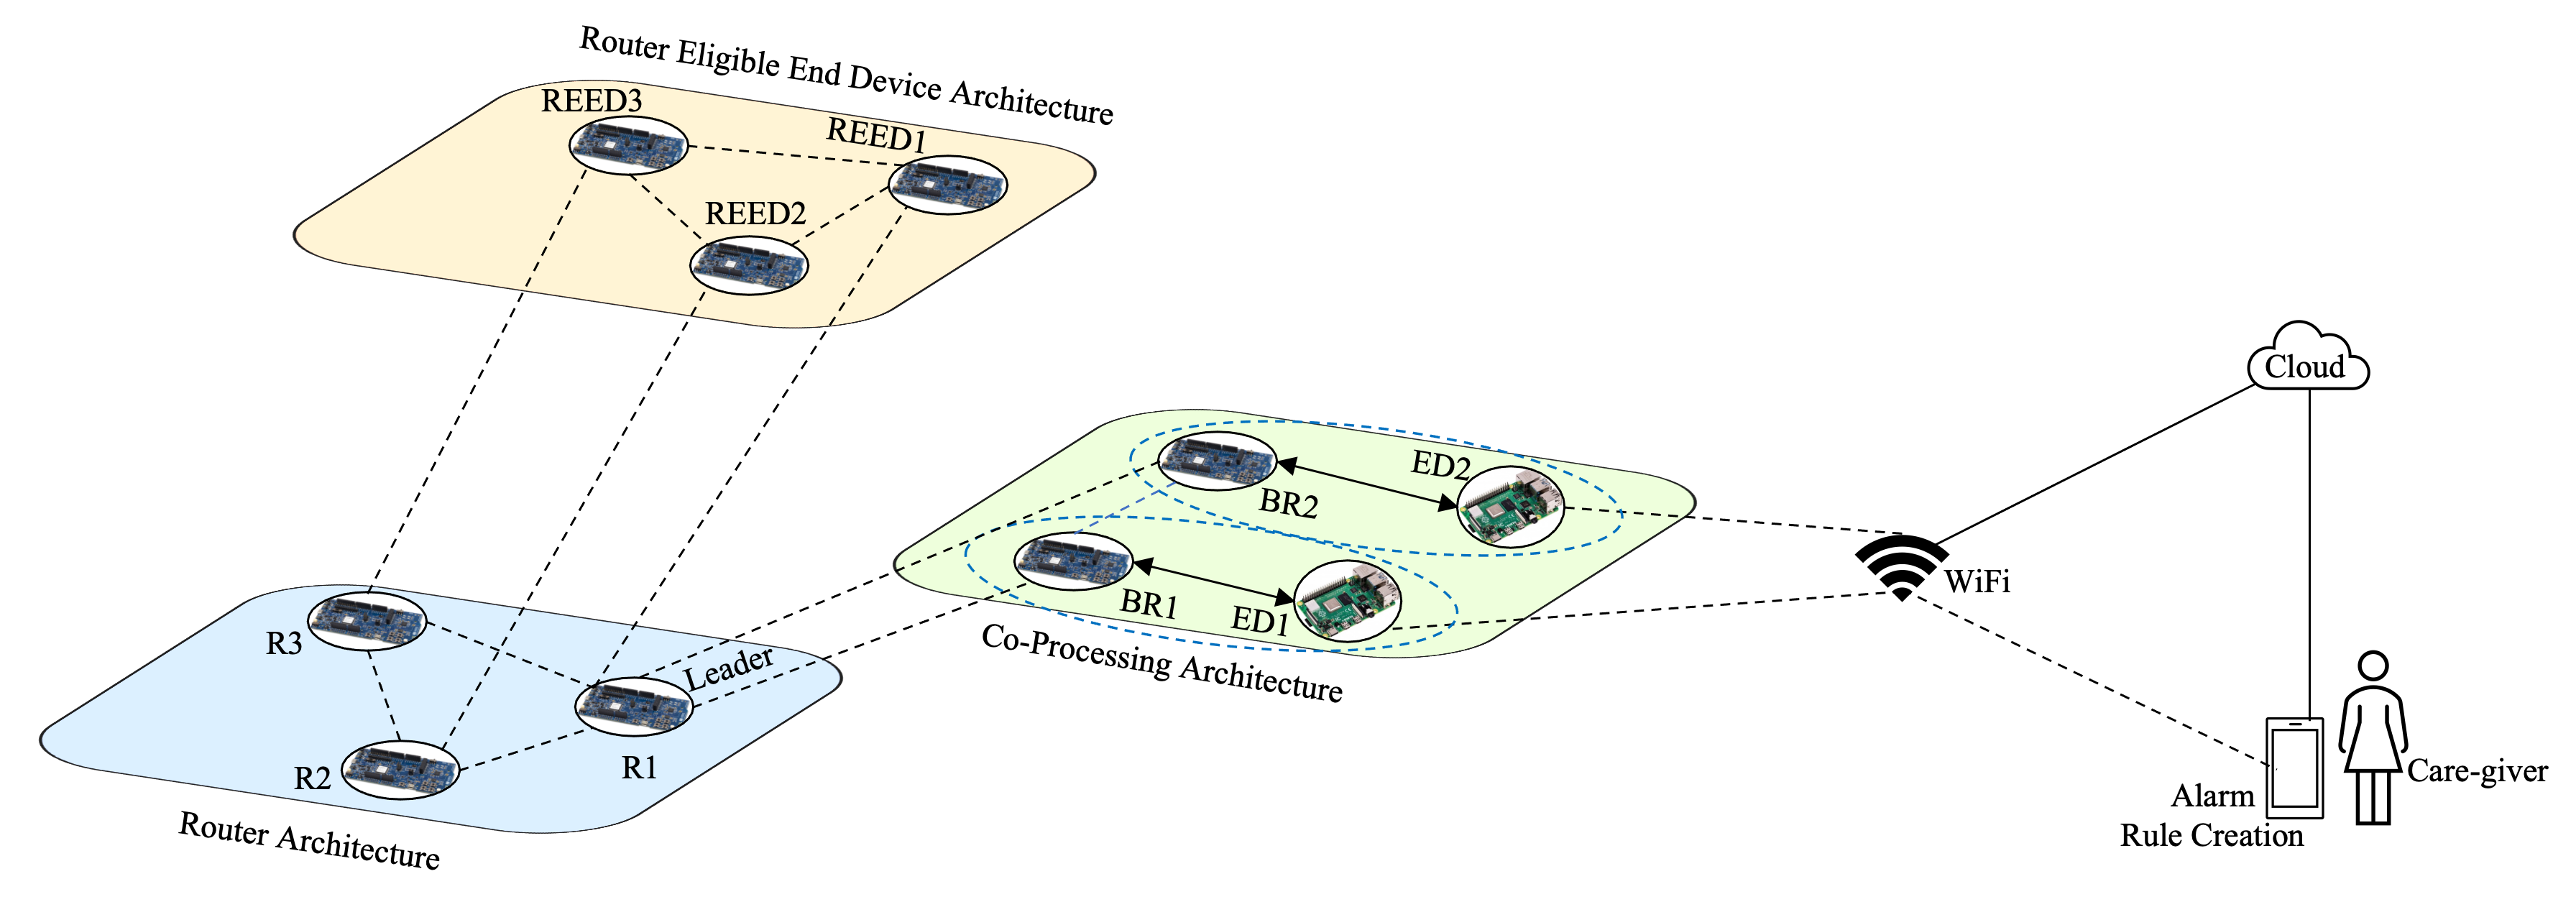
\includegraphics[width=0.8\textwidth]{images/research_design/prototype.png}
    \caption{Thread network topology of the prototype.}
    \label{fig:prototype}
\end{figure}

The construction process of the prototype involved several crucial steps, aimed at validating the output from MCM and GA and ensuring optimal network configuration:

\begin{enumerate}
    \item Customized nRF Thread Client and Server SDK to fit the needs for the research, selecting roles for each device and setting the transmission power output from both MCM and GA for optimal network configuration.
    \item Flashed each router with the Thread Server and each REED with the Thread Client customized SDK. In this configuration, routers acted as servers, while REEDs acted as clients. Communication between devices was bidirectional, with the clients having BLE enabled for multiprotocol support.
    \item Flashed the border router nodes with the Co-Processor setup provided by nRF. To enable the Raspberry Pi to act as an edge device, the OpenThread Radio Coprocessor (RCP) architecture was implemented.
    \item Turned on the devices one by one, noting that the first device activated in the network was most likely to become the leader, although leadership could change during the network's lifetime.
    \item Validated all the nodes by running multicast messages using Thread ICMP service. The ICMP service allowed sending echo requests (ping) to devices, activating their Thread antennas. This enabled testing the Thread connection, and devices could also reply \cite{Thread_Group_Fundamentals}.
    \item Validated the multiprotocol support connection by running a data flow from the ESP32 UWB and mobile devices to the REEDs through BLE, which then forwarded the data to the routers. This step ensured seamless communication between non-Thread devices and the Thread network.
    \item Monitored the network for stability and performance, adjusting settings to maintain optimal operation.
\end{enumerate}

Following these steps, the prototype was successfully constructed to apply the optimized settings obtained from the MCM and GA. The subsequent figure presented a real-world Thread network prototype setup from the lab setup. The image provided a clear view of the nRF52840-based Thread nodes, Raspberry Pi as the edge device, and the border router setup with the dongle. It also showcased the development kits used for routers and REEDs.

\begin{figure}[H]
    \centering
    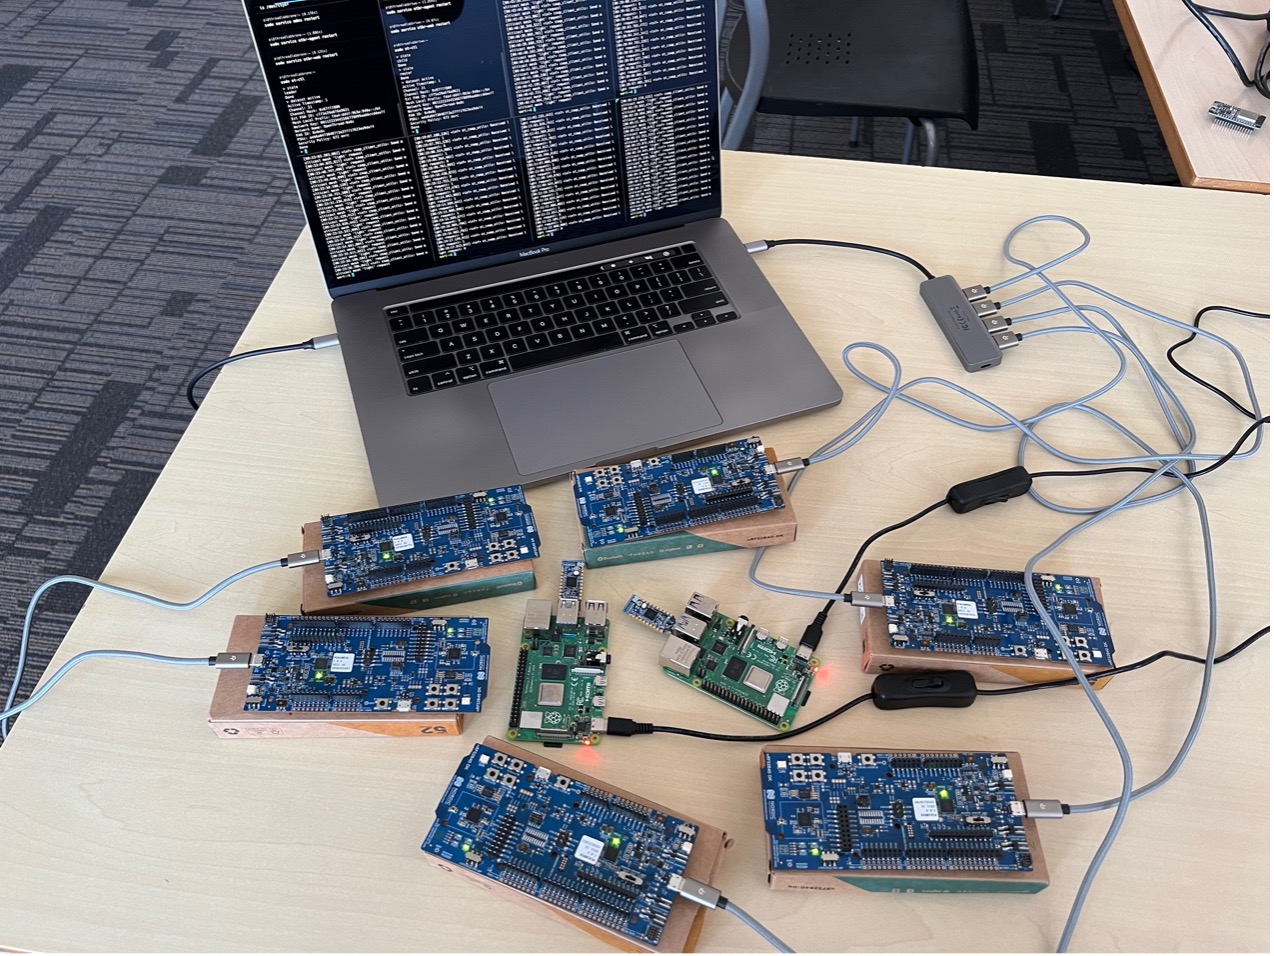
\includegraphics[width=0.8\textwidth]{images/research_design/prototype_setup.jpg}
    \caption{Thread network prototype setup in the lab.}
    \label{fig:prototype_setup}
\end{figure}

\section{Data Collection}

The data collection process aimed to validate and compare the solutions from MCM and GA against the maximum mode by measuring power consumption in each device of the built prototype. Utilizing the nRF Power Profiler Kit II, which offers Current $\left(ma\right)$ measurement at 100,000 samples per second, allowed for accurate power consumption measurements across various scenarios, locations, network activities, optimization modes, and durations. This approach provided insights into the effectiveness of the optimization techniques in both controlled and real-world settings while avoiding excessive data that would have complicated the analysis process.

\begin{enumerate}
    \item \textbf{Method}: Power consumption was measured in two primary scenarios - Maximum and Optimized. The maximum scenario represented the baseline power consumption, where no optimization techniques were applied. The optimized scenario measured power consumption after implementing the MCM and GA optimization techniques.
    \item \textbf{Location}: Measurements were conducted in two different locations - Lab and Home. The lab setting, smaller in size compared to the home location, allowed for controlled environments and reproducible results. The home setting provided a real-world context with a larger area, helping to understand the performance of the Thread network in everyday IoT applications. The following images show the Euclidean distance matrix from two different locations to share a clear view of the distance between each device in the two locations.
    \begin{figure}[H]
        \centering
        \begin{minipage}{0.5\textwidth}
            \centering
            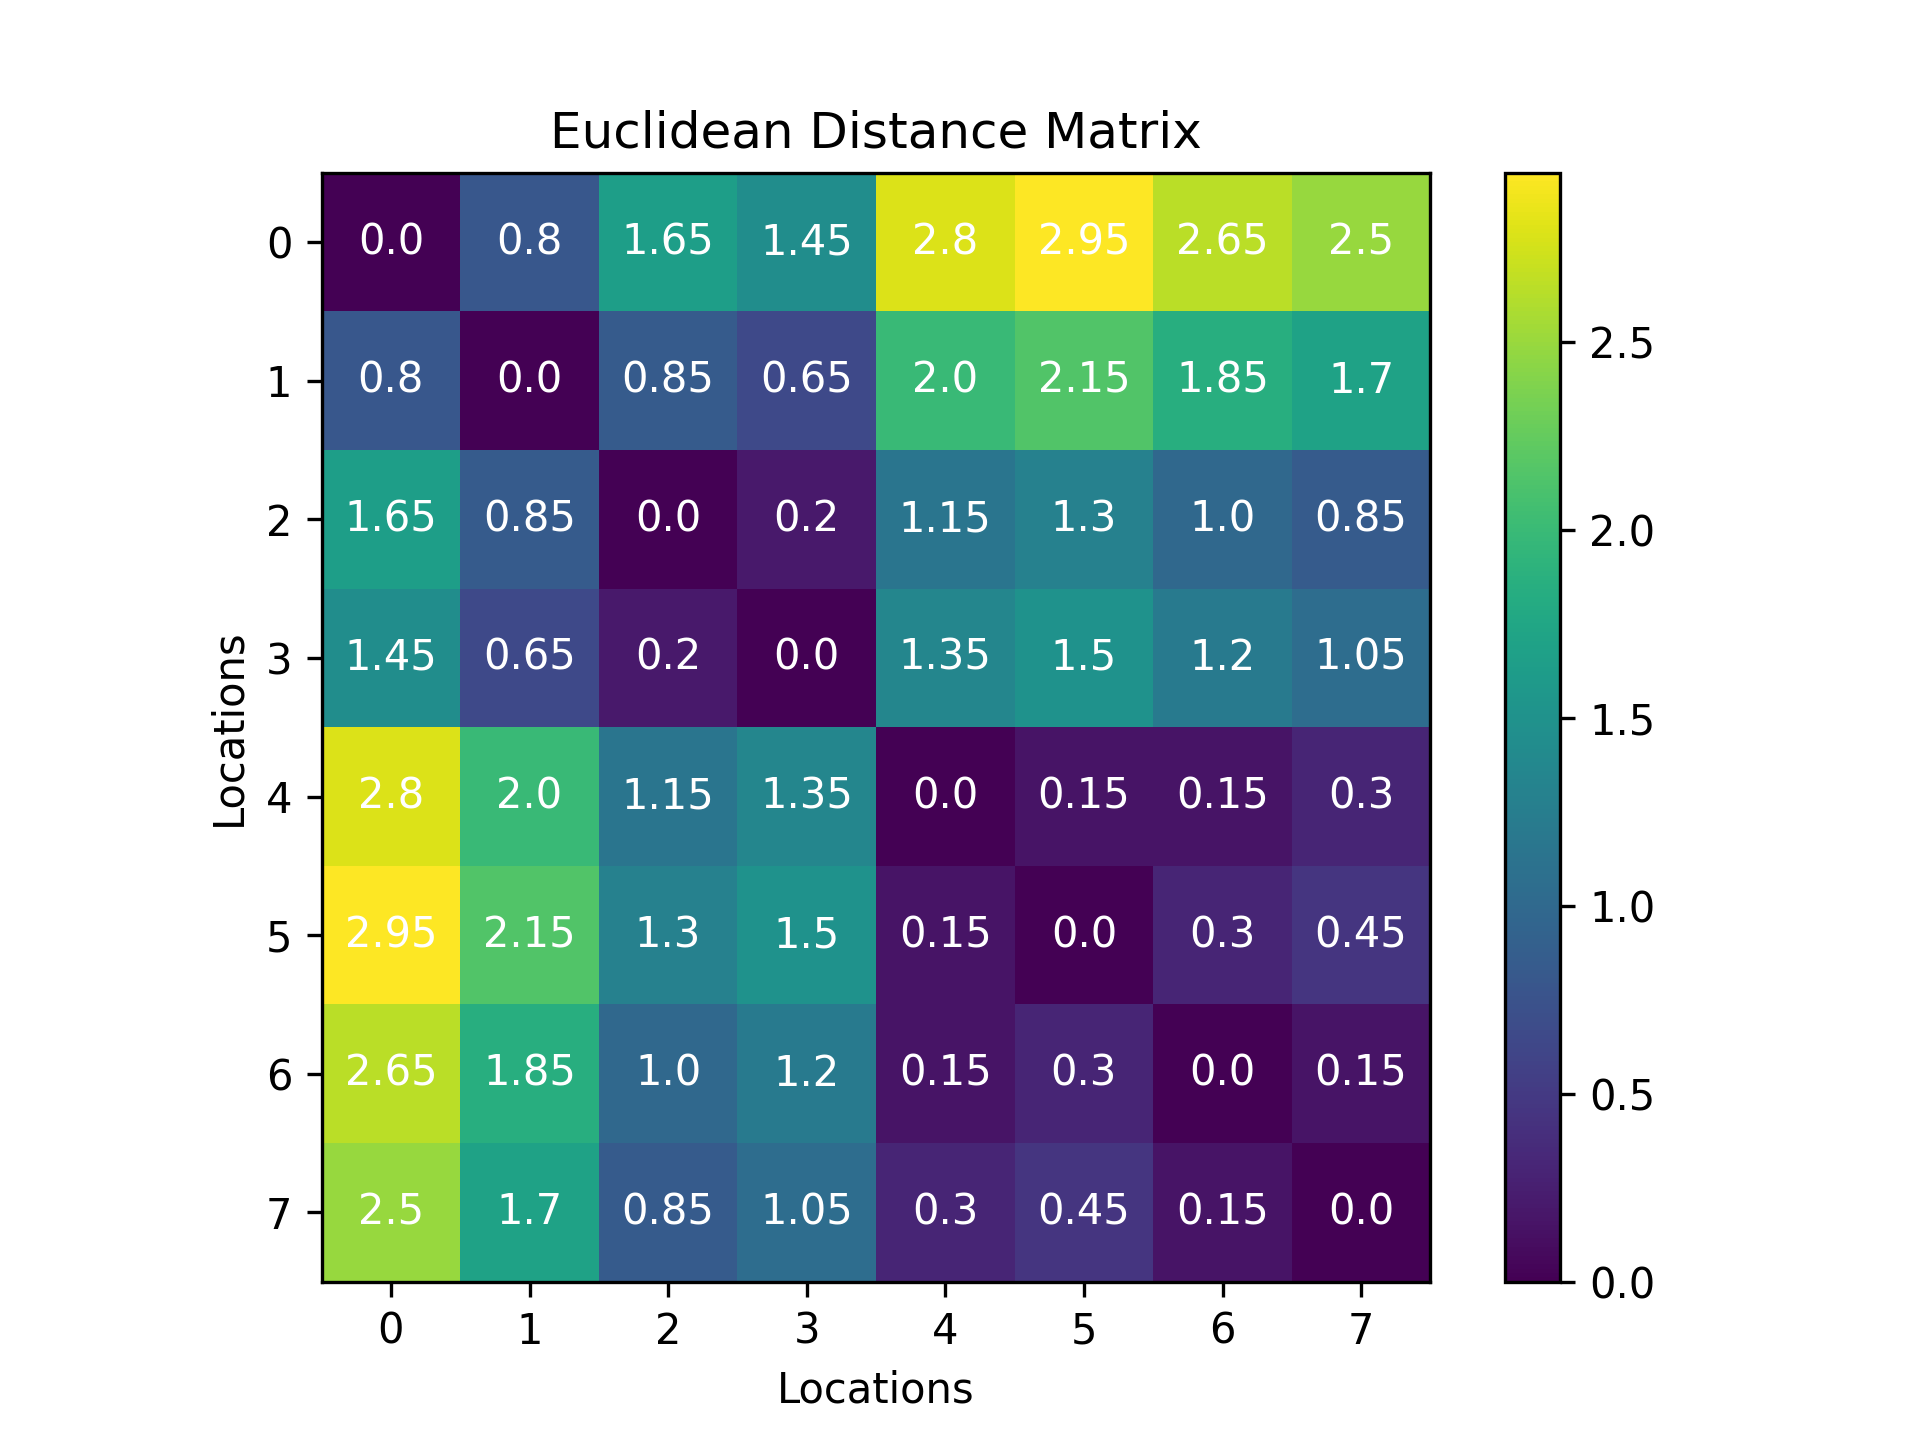
\includegraphics[width=1\textwidth]{images/research_design/distance_matrix_lab.png}
            \captionof{figure}{Distance matrix for lab.}
            \label{fig:distance_matrix_lab}
        \end{minipage}%
        \begin{minipage}{0.5\textwidth}
            \centering
            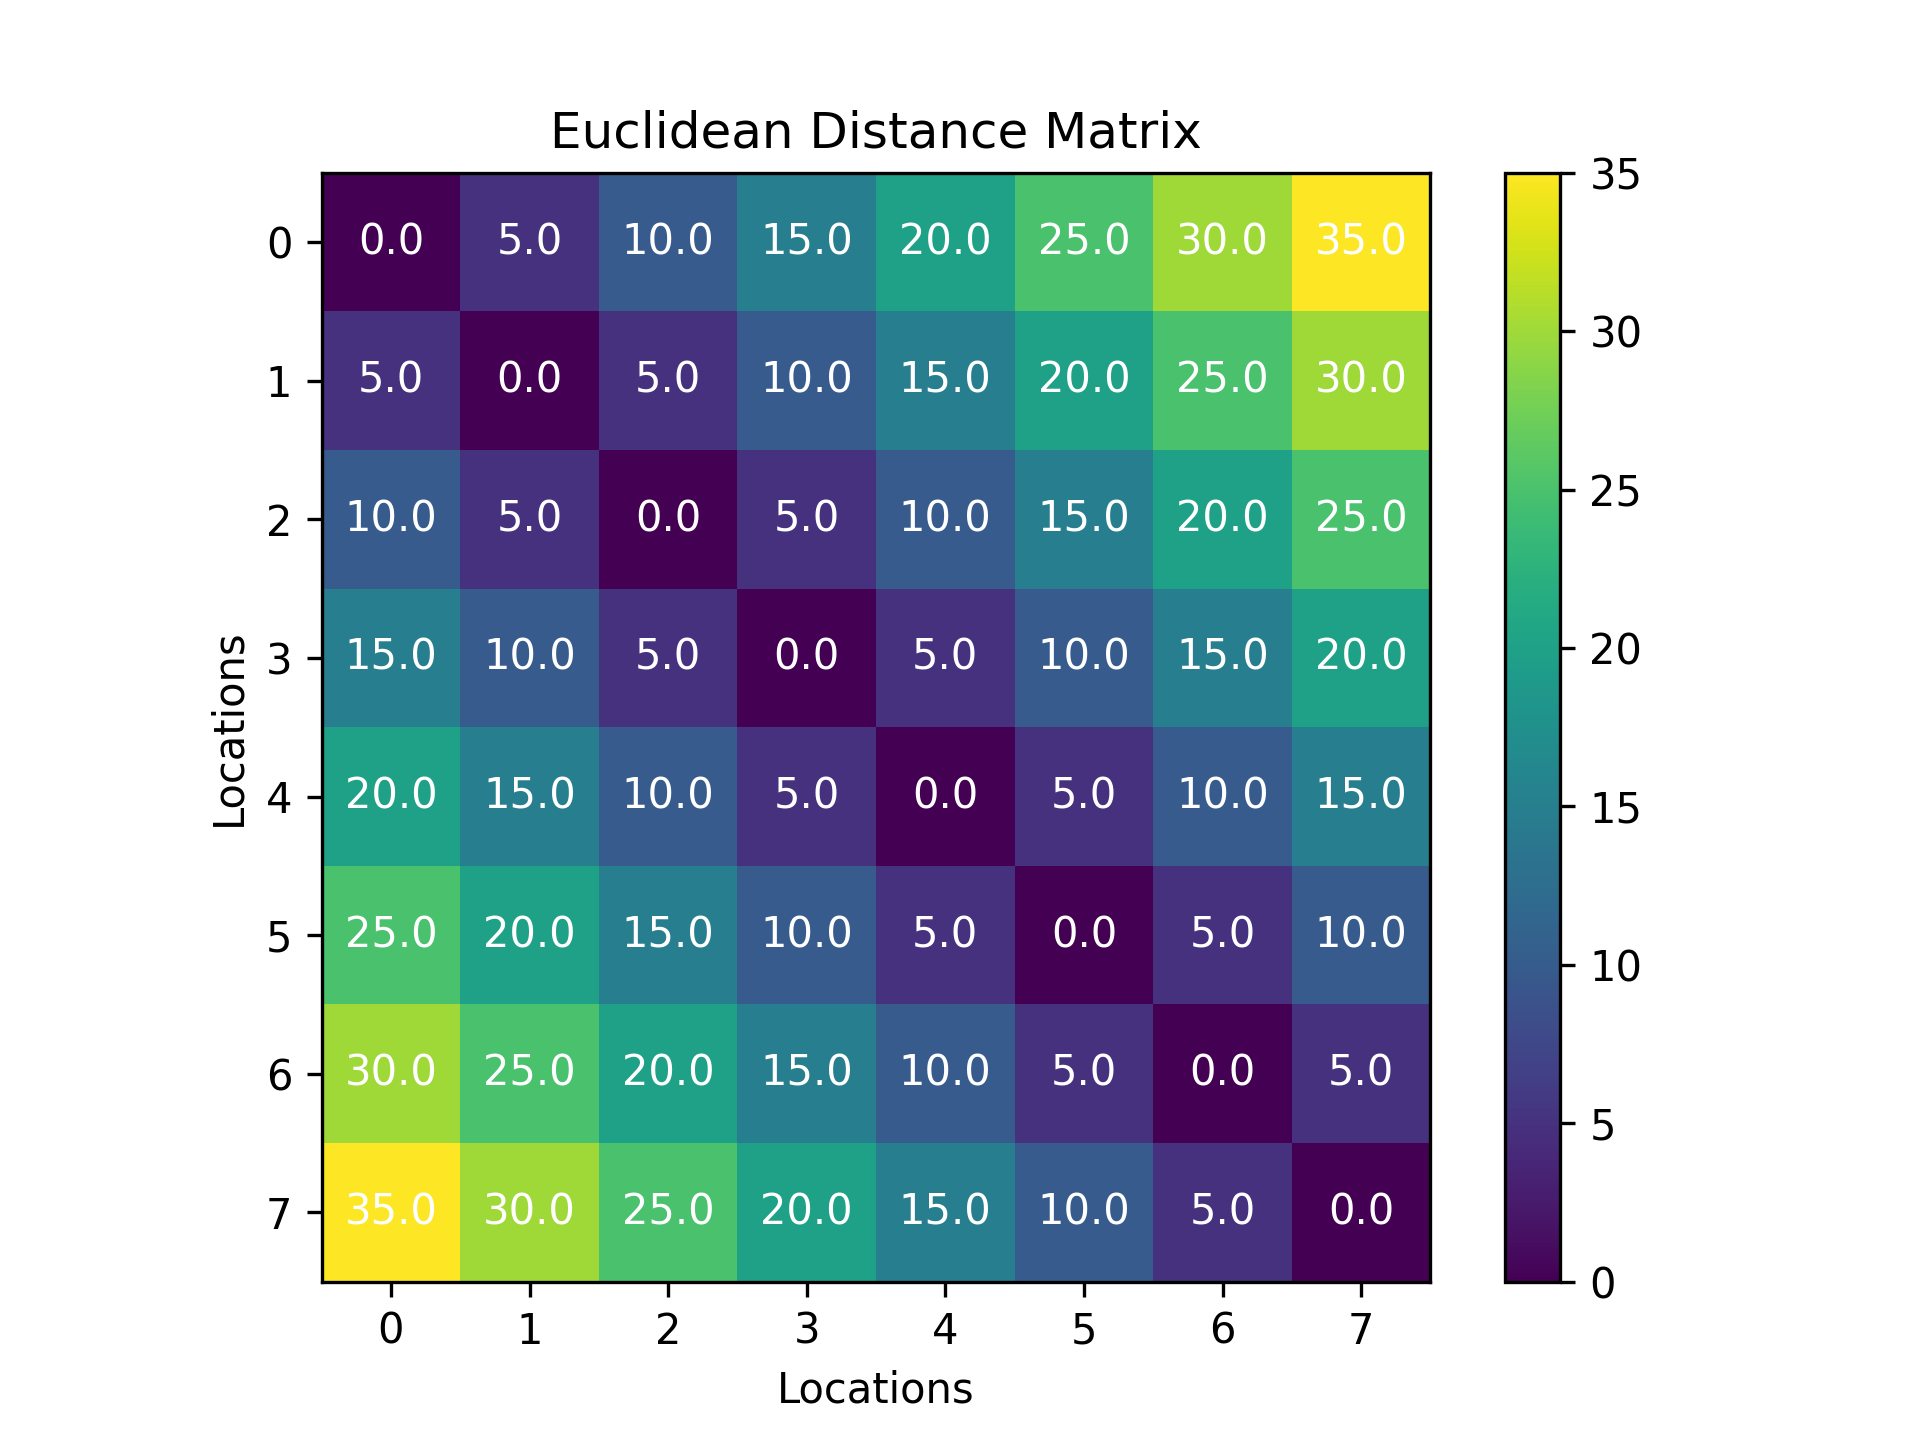
\includegraphics[width=1\textwidth]{images/research_design/distance_matrix_home.png}
            \captionof{figure}{Distance matrix for home.}
            \label{fig:distance_matrix_home}
        \end{minipage}
    \end{figure}
    \item \textbf{Type}: Power consumption measurements were also conducted based on the type of network activity. The No Sensor scenario represented a Thread network with no active sensors, while the Ping scenario simulated data exchange between nodes, resembling real IoT network behavior \cite{Thread_Group_Fundamentals}.
    \item \textbf{Mode}: The project compared the effectiveness of MCM and GA optimization techniques. The MCM mode measured power consumption based on network configurations optimized using the Monte Carlo Method. The GA mode measured power consumption with network configurations optimized using the Genetic Algorithm.
    \item \textbf{Duration}: Power consumption measurements were conducted for different durations - 60 seconds in the Lab location and 300 seconds in the Home location. This variation in duration helped in understanding the impact of time on power consumption in different environments.
    \item \textbf{Ping}: In the lab location, 50 pings were sent within the 60-second duration, whereas in the home location, 290 pings were sent during the 300-second duration. This distinction helped analyze the impact of network activity on power consumption in both controlled and real-world settings.
\end{enumerate}

Following the data collection steps, two images are provided to illustrate the process of collecting power consumption data from the nRF52840 DK using the PPKII. These images offer a visual representation of the setup and the data collection process, giving a clearer understanding of the experimental context and the methods used for obtaining the power consumption measurements.

\begin{figure}[H]
    \centering
    \begin{minipage}[t]{0.45\textwidth}
        \centering
        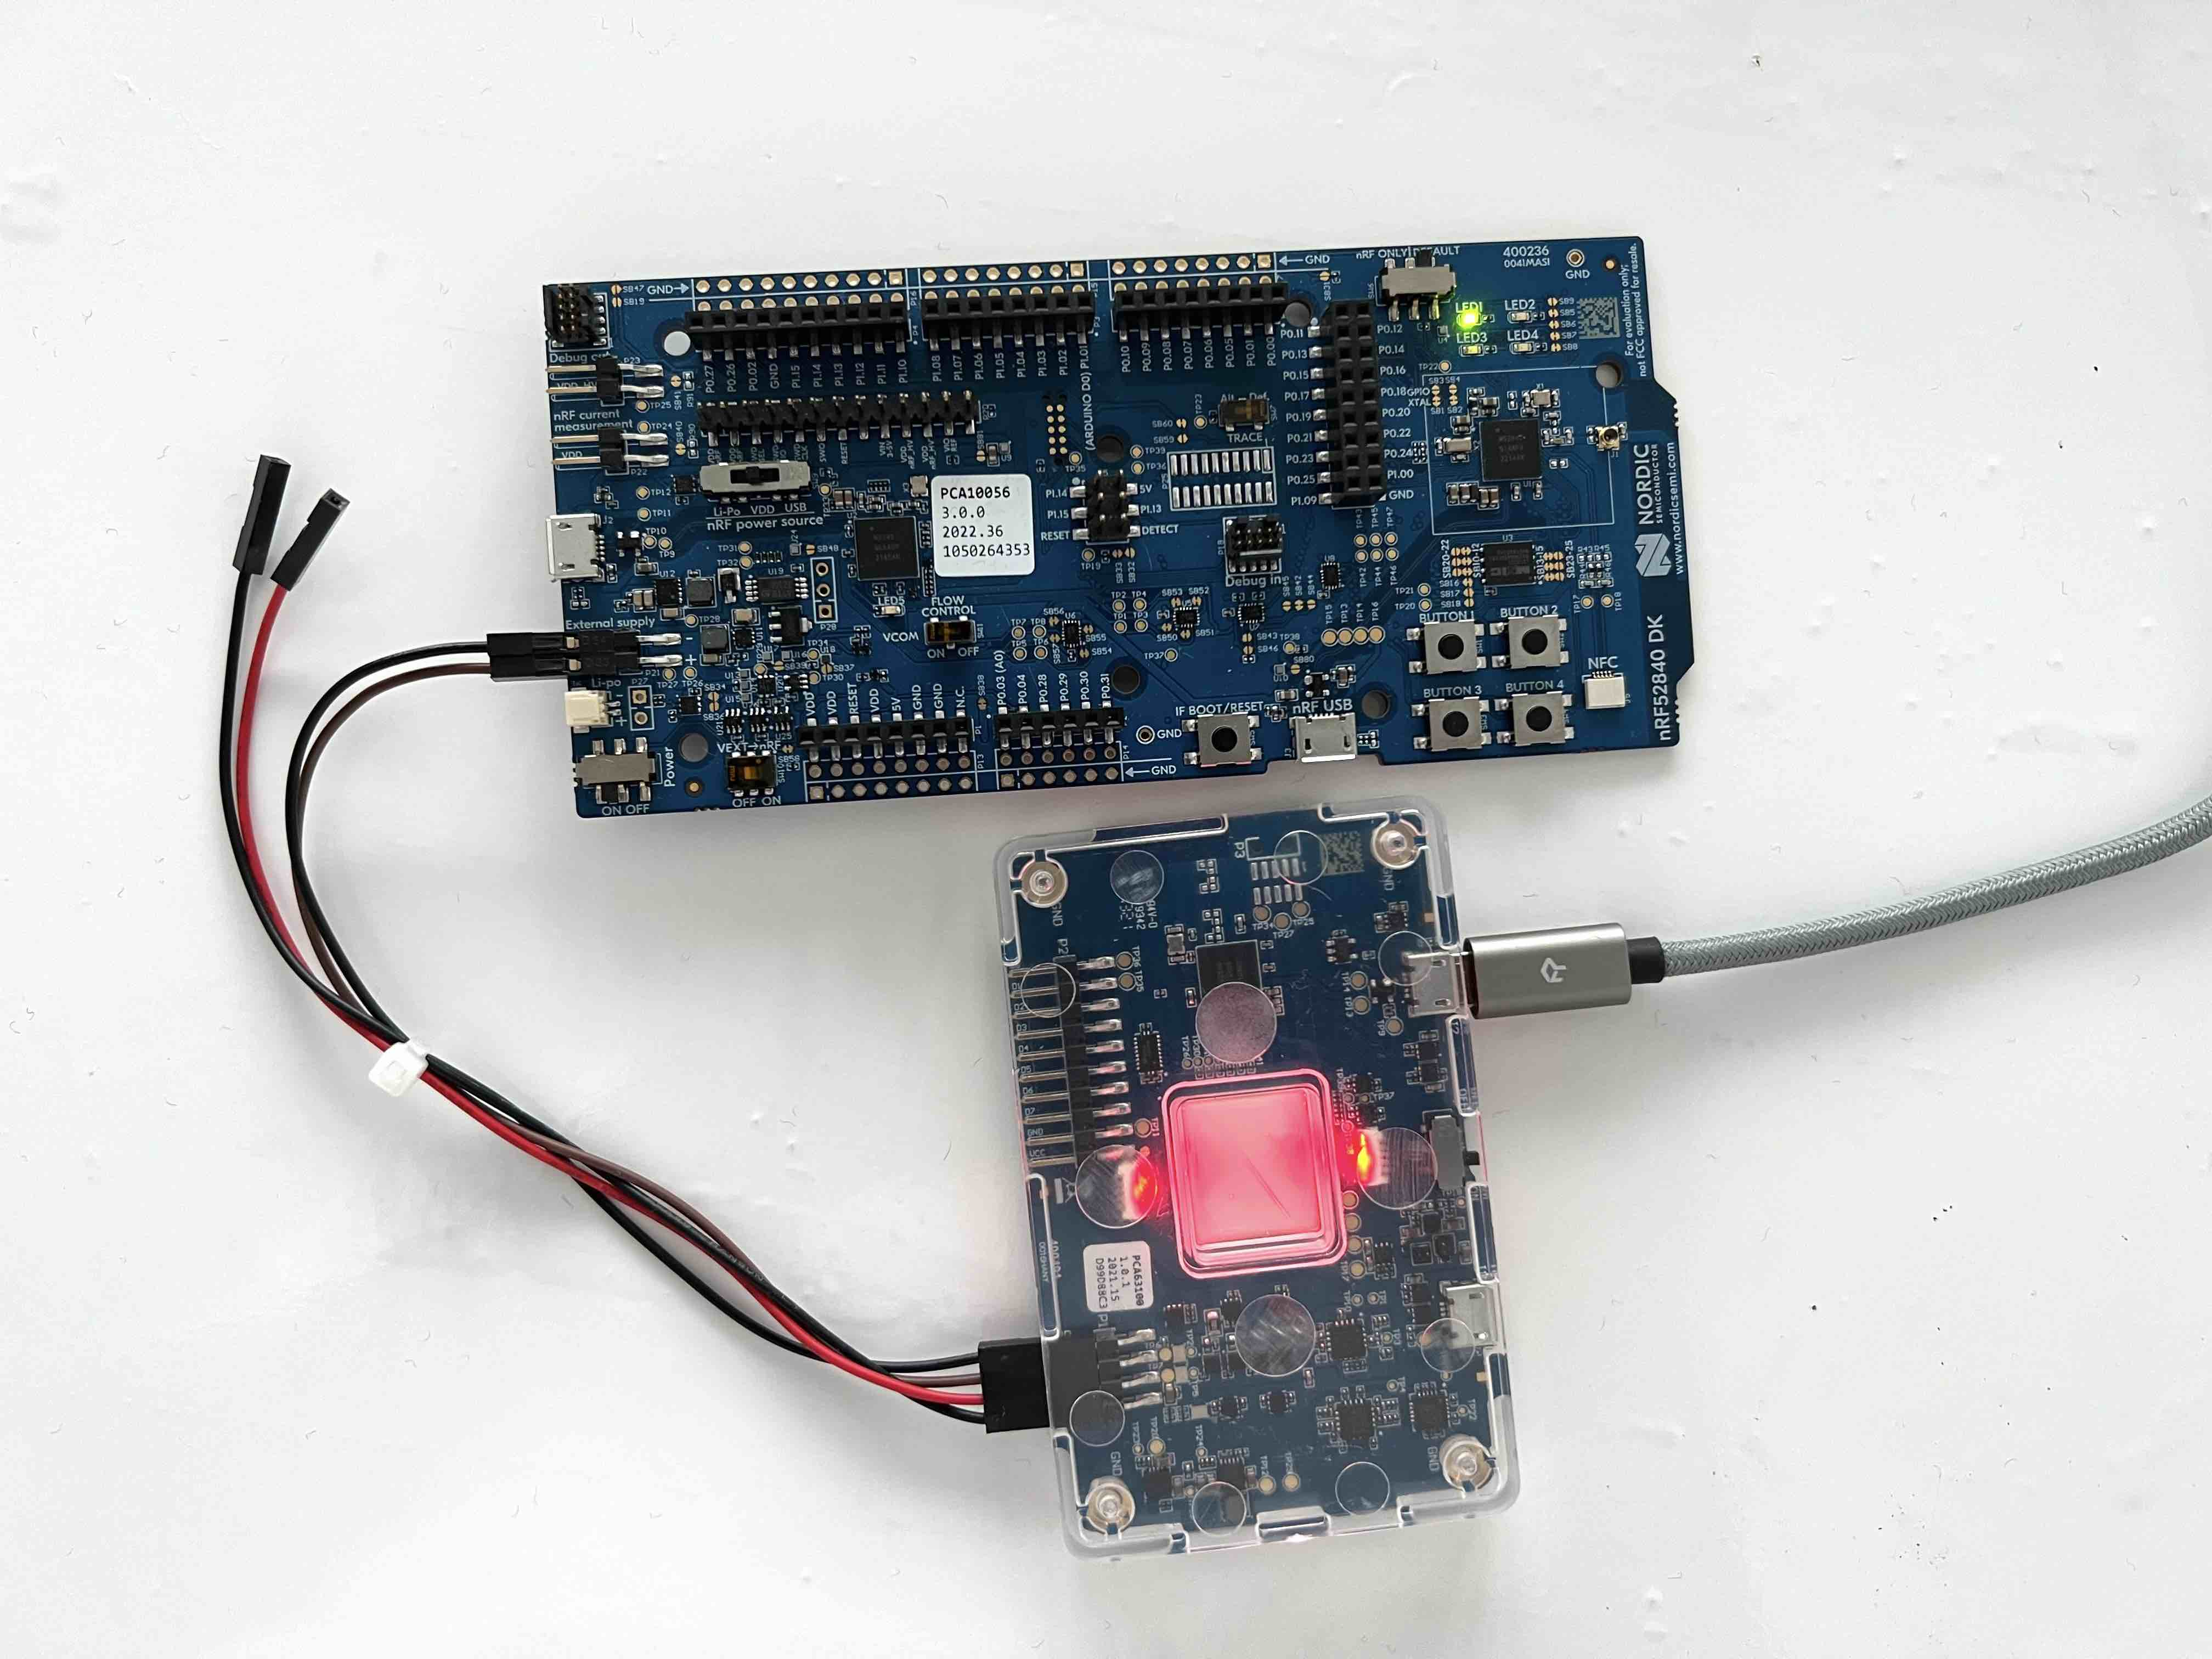
\includegraphics[width=1\linewidth]{images/research_design/PPK2_Router.jpg}
        \captionof{figure}{PPK II connected to a router.}
        \label{fig:router_source_meter}
    \end{minipage}\hfill
    \begin{minipage}[t]{0.45\textwidth}
        \centering
        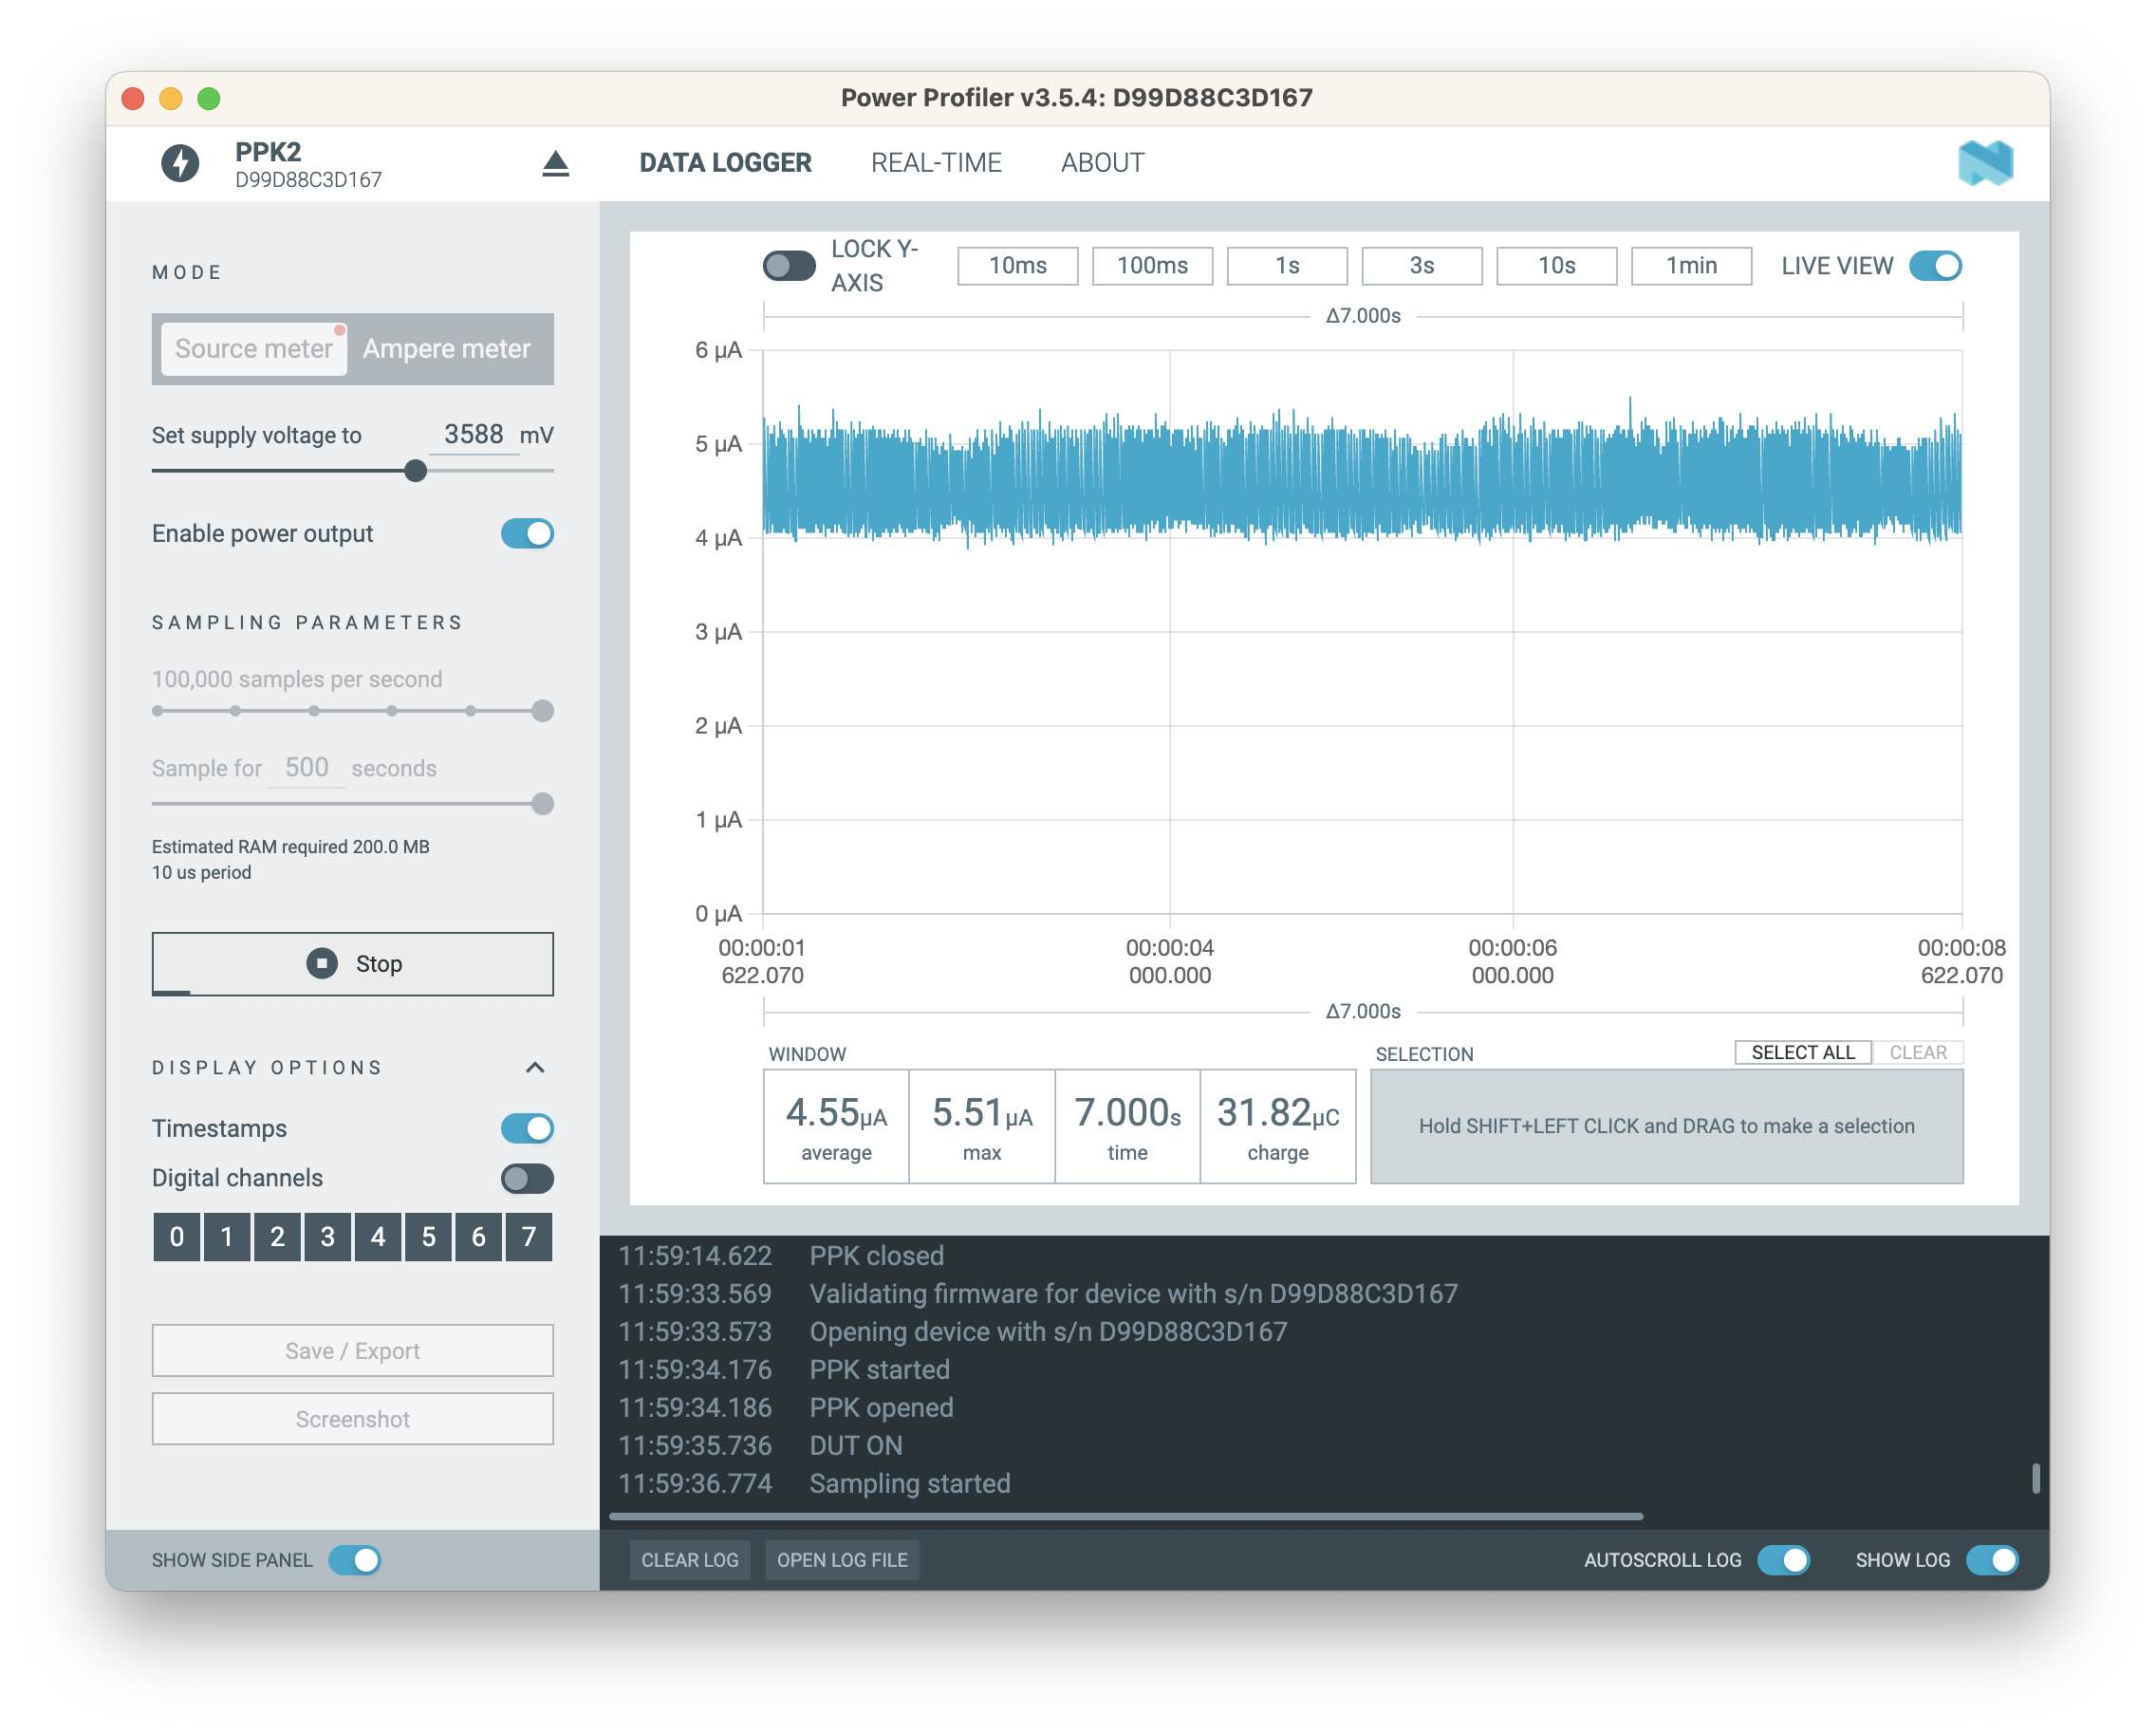
\includegraphics[width=1\linewidth]{images/research_design/PPK2_SDK.jpg}
        \captionof{figure}{PPK II software in source meter mode.}
        \label{fig:ppk2_source_meter}
    \end{minipage}
\end{figure}
